\documentclass[12pt]{article}

\usepackage{amsmath}
\usepackage{amsfonts}
\usepackage{graphicx}

\title{CAGD - Abgabe 1: Results} 
\author{Stefan Zaufl \\ Hanna Huber}

\begin{document}
\maketitle

\section{Aufgabe 1}

\begin{figure}
\centering{
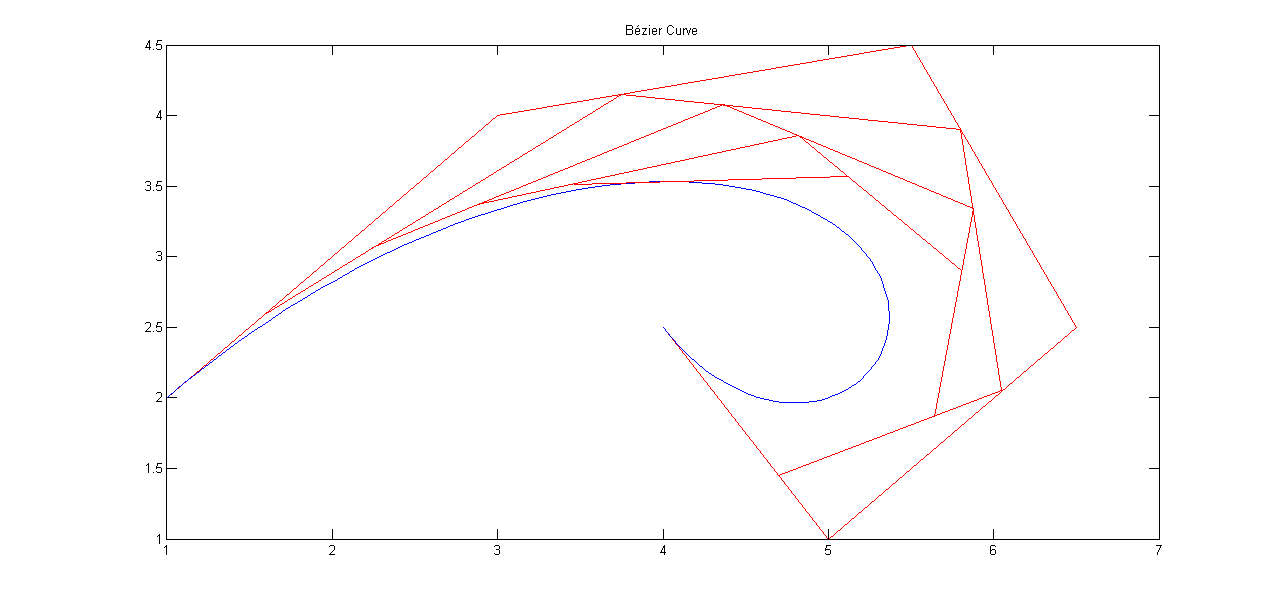
\includegraphics[width=\textwidth]{1a.png}}
\caption{The algorithm of de Casteljau for t=0.3}
\label{fig:1a}
\end{figure}

The algorithm of de Casteljau is illustrated in Figure~\ref{fig:1a}.

\begin{figure}
\centering{
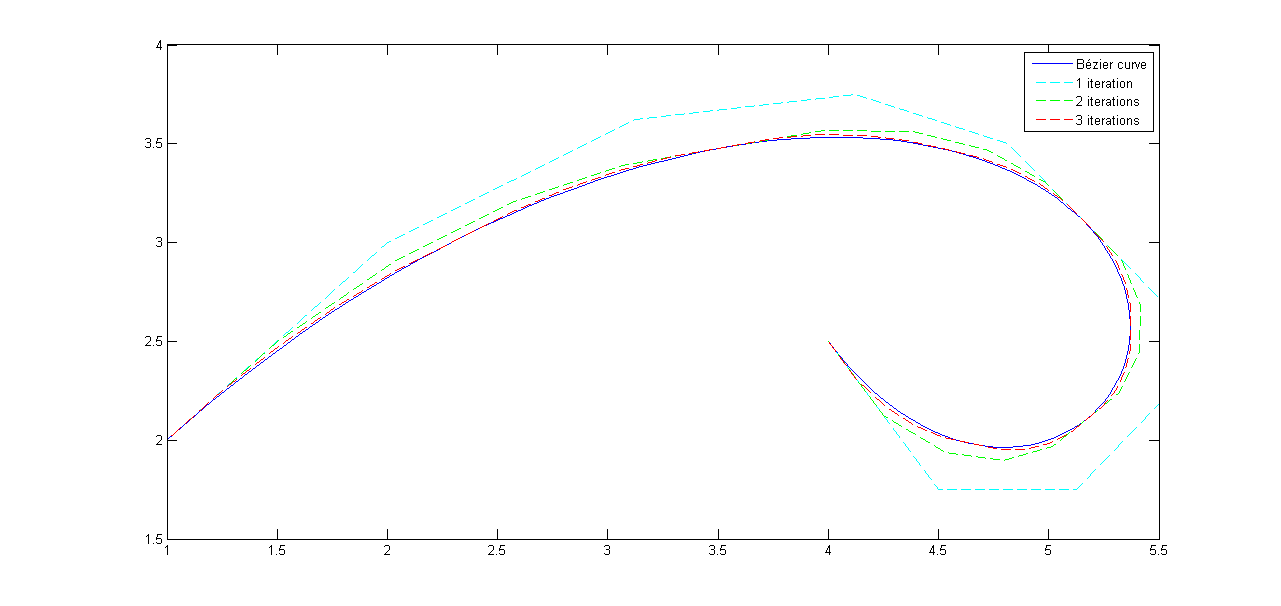
\includegraphics[width=\textwidth]{1b.png}}
\caption{Comparison of the Bezier curve and its approximations applying the algorithm of de Casteljau one, two and three times, respectively.}
\label{fig:1b}
\end{figure}


\section{Aufgabe 2}

\end{document}